\chapter{Methodology}

We developed the ROAD-Waymo pipeline through controlled changes to a replicated joint detector. Detector replacement and score transfer are followed by direct region-feature classification and learned composition. This chapter defines these completed methods and their shared evaluation protocol. The resulting rare-composition gap motivates the semantic-classifier study in Chapter 5.

The completed stages share the benchmark label layout and evaluator. Changes in boxes, representation, classifier, and composition are described explicitly so that improvements are attributed only to the intervention supported by a comparison.

\section{Dataset, Prediction Targets, and Evaluation}

The study uses the ROAD-Waymo training and validation partitions \cite{road-waymo}: 600 training videos and 198 validation videos. The publicly unannotated test partition is outside the reported evaluation. Dataset counts and tail membership refer to the local annotation release and project audit, rather than substituting aggregate counts reported for other releases.

Each candidate is associated with the score groups in Table~\ref{tab:2}. Agentness is a separate object-presence score. Action and location are multi-label tasks, and each composition is a benchmark-defined combination. The total is 1 + 10 + 22 + 16 + 49 + 86 = 184.

\begin{table}[htbp]
\centering
\caption{Prediction groups and output dimensions.}
\label{tab:2}
\begin{singlespace}
\begin{tabular}{@{}lcc@{}}
\toprule
\textbf{Prediction groups} & \textbf{Dimensions} & \textbf{Meaning} \\
\midrule
Agentness + agent & 1 + 10 & Presence + identity \\
Action + location & 22 + 16 & Activity + position \\
Duplex + triplet & 49 + 86 & Event compositions \\
Total & 184 & Six output groups \\
\bottomrule
\end{tabular}
\end{singlespace}
\end{table}

All completed-stage comparisons use frame-level mean average precision at IoU 0.5 through the baseline repository’s evaluator. Predictions are ranked by class and matched to ground truth on each frame. AP summarizes the precision--recall curve; mAP averages class APs. The reported comparison is restricted to 36,717 validation frames shared by the detection sources and required feature records.

Figure~\ref{fig:frame-map} shows how a scored box contributes to this metric. For each class, the evaluator processes detections in descending score order within a frame and matches each detection to an available ground-truth box of that class when IoU is at least 0.5. Each ground-truth box can be matched once. Unmatched detections, including duplicate detections after a ground-truth box has been consumed, count as false positives. The evaluator then ranks detections across the selected frames to obtain a precision--recall curve. It integrates the interpolated precision envelope at changes in recall and averages AP over the classes in the reported group. This follows the detection-evaluation principles of PASCAL VOC \cite{voc}; the actual implementation is the ROAD baseline evaluator \cite{road}.

\begin{figure}[htbp]
\centering
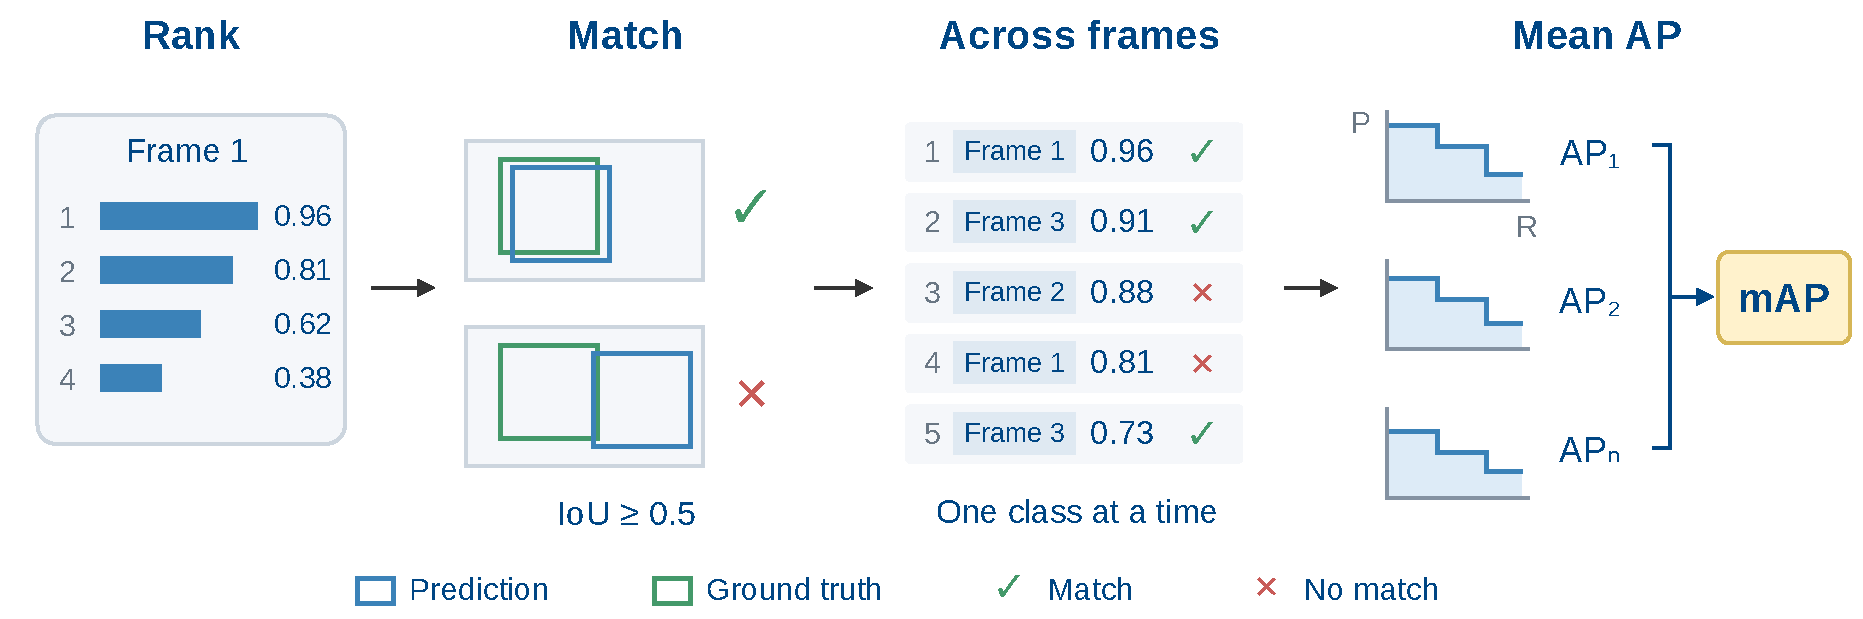
\includegraphics[width=\textwidth,height=0.60\textheight,keepaspectratio]{Fig/frame-map.pdf}
\caption[Frame-level average-precision evaluation.]{Frame-level average-precision evaluation. Scores and curves are schematic; matching is class-specific and restricted to the same frame.}
\label{fig:frame-map}
\end{figure}

“Full-candidate” denotes a broad low-threshold candidate pool, capped at 300 per frame, rather than exhaustive boxes or every annotated validation frame. Stage 0 uses its own candidates. Stages 1--3 share YOLO candidates. The original baseline validation path filters scores per class and per frame; the comparison path assembles predictions from saved dumps, including temporally averaged agentness for baseline candidate selection. Thus, using the same metric code alone does not make different filtering protocols equivalent.

The primary metric is f-mAP, not tube-level video-mAP. No test-server result is claimed. Training labels define tail membership, while validation predictions determine AP. The same tail class lists are used for every compared model.

\section{Replicated Joint Baseline}

The starting point is 3D-RetinaNet, which processes eight-frame clips through an I3D backbone and feature pyramid before predicting box offsets and class scores \cite{road}. Localization and classification share a learned representation. The replicated checkpoint provides both the baseline detections and the frozen visual backbone used in the early hybrid stages.

Two evaluations are distinguished. The earlier baseline validation produced 17.76\% agent and 9.17\% triplet f-mAP. The Stage 0 row in this proposal’s shared-frame comparison is 16.67\% agent and 7.54\% triplet f-mAP. The difference reflects evaluation conditions, including frame selection and candidate filtering; the numbers are not interchangeable.

Figure~\ref{fig:2} gives the Stage 0 data flow. The trained baseline predicts its own boxes and event scores; later hybrid stages reuse its frozen backbone or detections.

\begin{figure}[htbp]
\centering
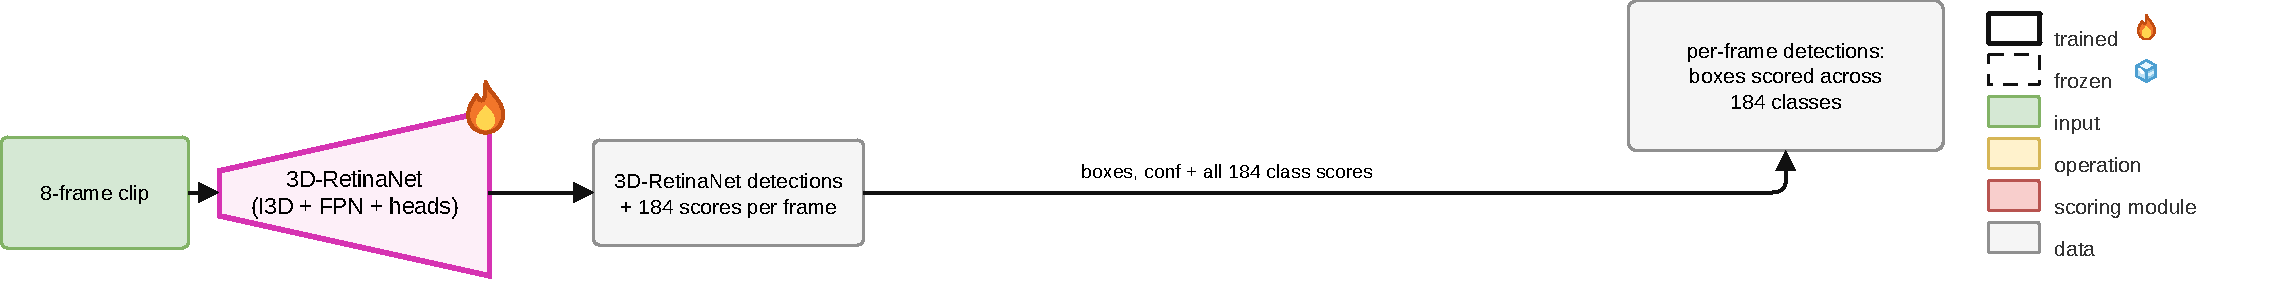
\includegraphics[width=\textwidth,height=0.68\textheight,keepaspectratio]{Fig/stage0-baseline.pdf}
\caption{Stage 0 joint detection and classification baseline.}
\label{fig:2}
\end{figure}

Figure~\ref{fig:3} details the ResNet50-I3D feature pyramid and detection subnets in the replicated 3D-RetinaNet. RetinaNet introduced focal loss for dense one-stage detection \cite{focal-loss}; ROAD adapts this architecture to video road-event detection \cite{road}.

\begin{figure}[htbp]
\centering
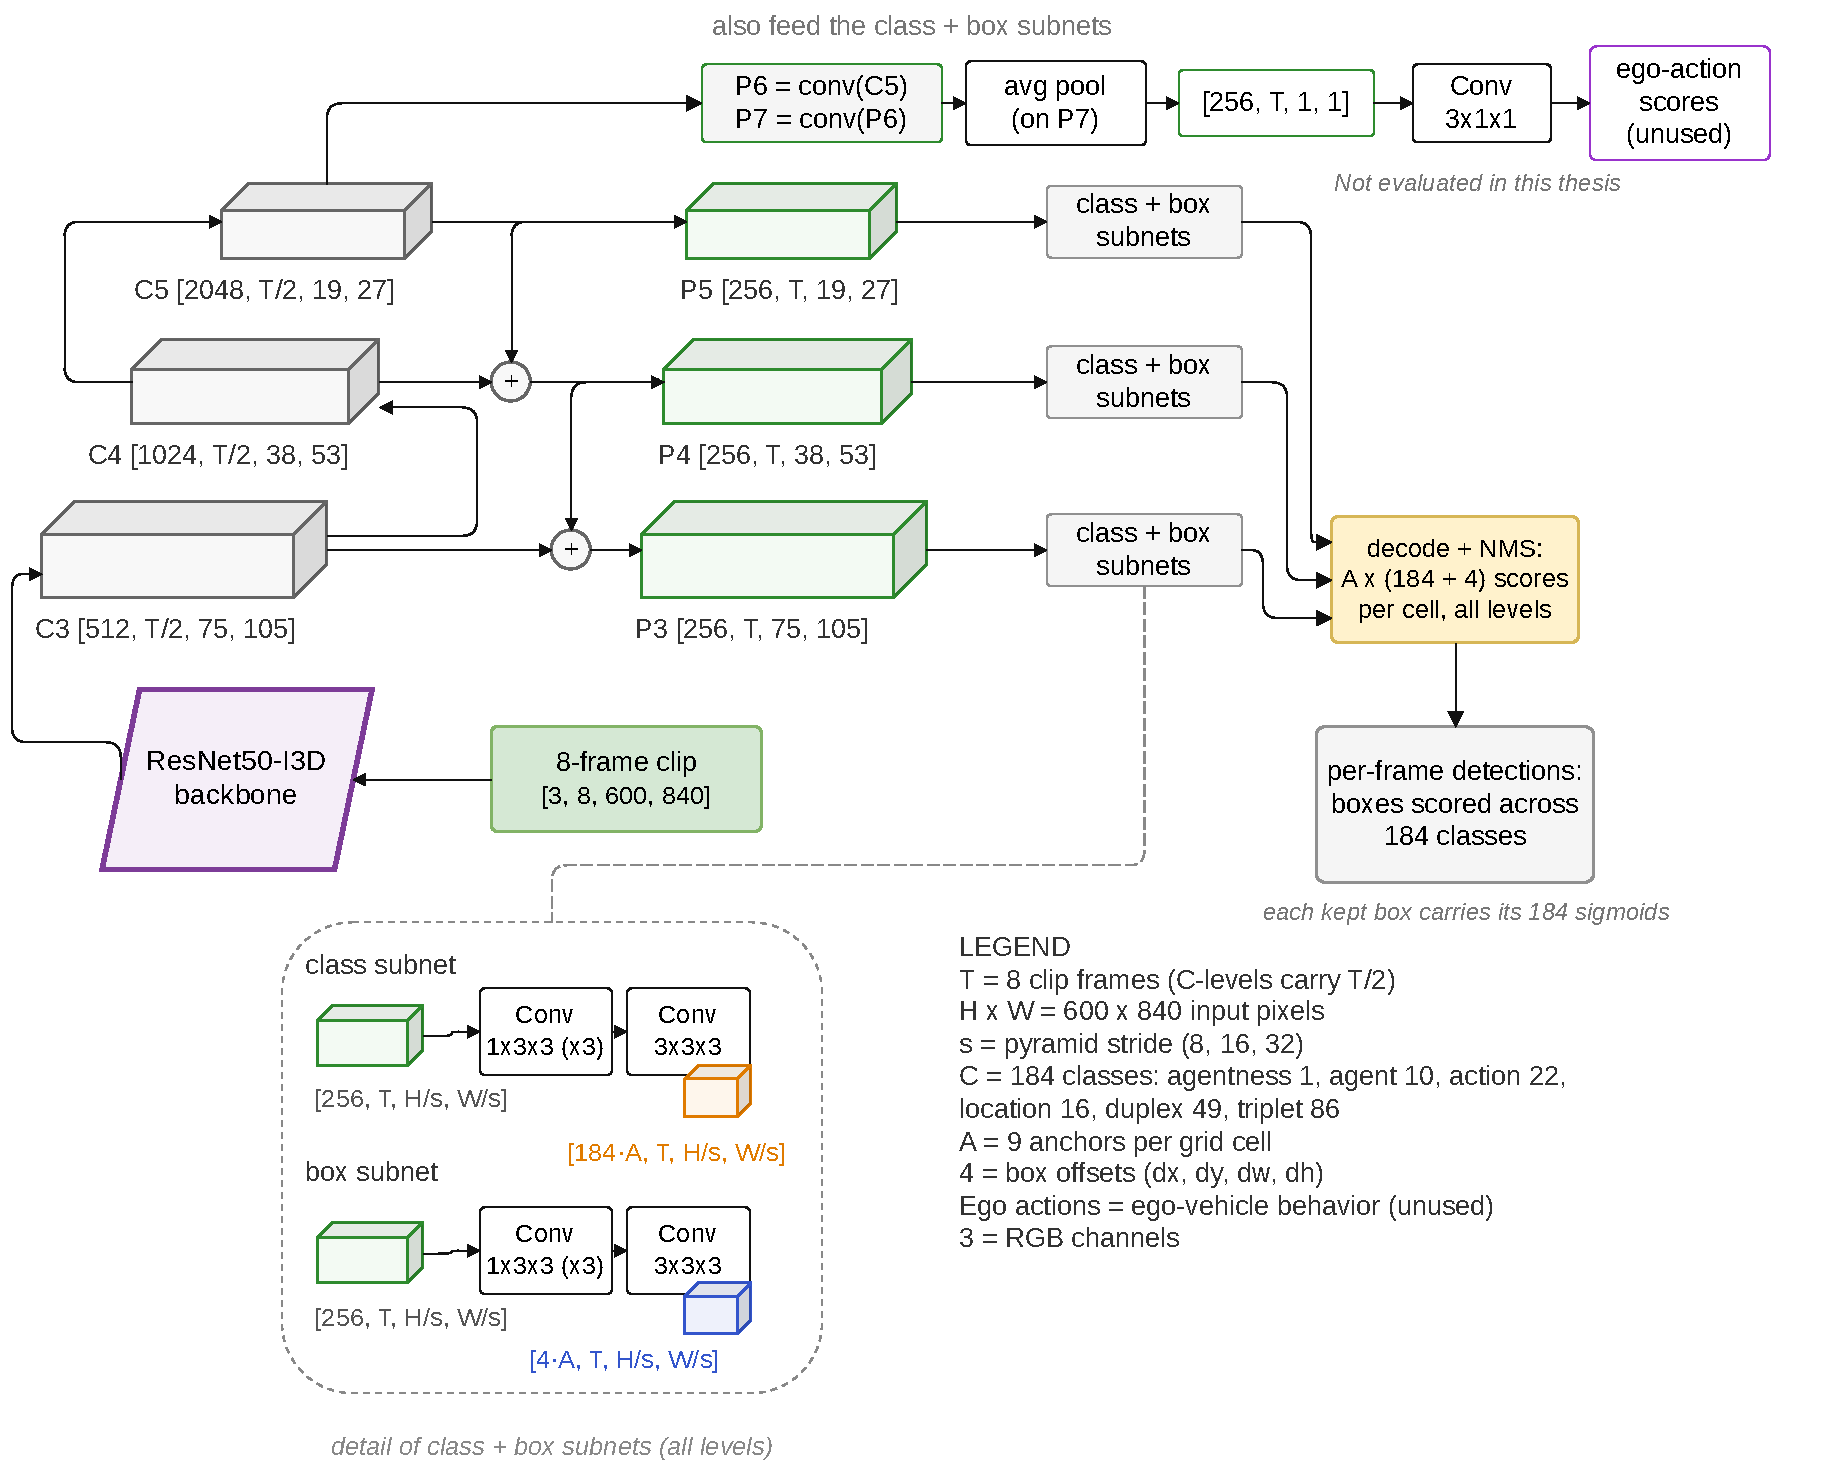
\includegraphics[width=\textwidth,height=0.68\textheight,keepaspectratio]{Fig/retinanet3d.pdf}
\caption{Replicated 3D-RetinaNet with a ResNet50-I3D backbone and feature pyramid.}
\label{fig:3}
\end{figure}

\section{Detector Replacement and Score Transfer}

YOLOv8x \cite{yolov8}, fine-tuned on ROAD-Waymo agent classes with a 1280-pixel input setting, supplies candidate boxes, confidence, and hard agent identity. The project training configuration follows the ECCV 2024 Track-1 recipe with documented implementation choices; the selected checkpoint is the recorded epoch-1 model. Candidate generation uses confidence 0.001, NMS IoU 0.7, and at most 300 detections per frame.

Figure~\ref{fig:4} details the YOLOv8x detector used for agent localization. The 1280 \(\times\) 1920 annotation identifies source-frame dimensions; the implementation applies Ultralytics resizing and letterboxing with imgsz = 1280. The 50-epoch setting describes the configured training recipe, while the reported comparison uses the selected epoch-1 checkpoint.

\begin{figure}[htbp]
\centering
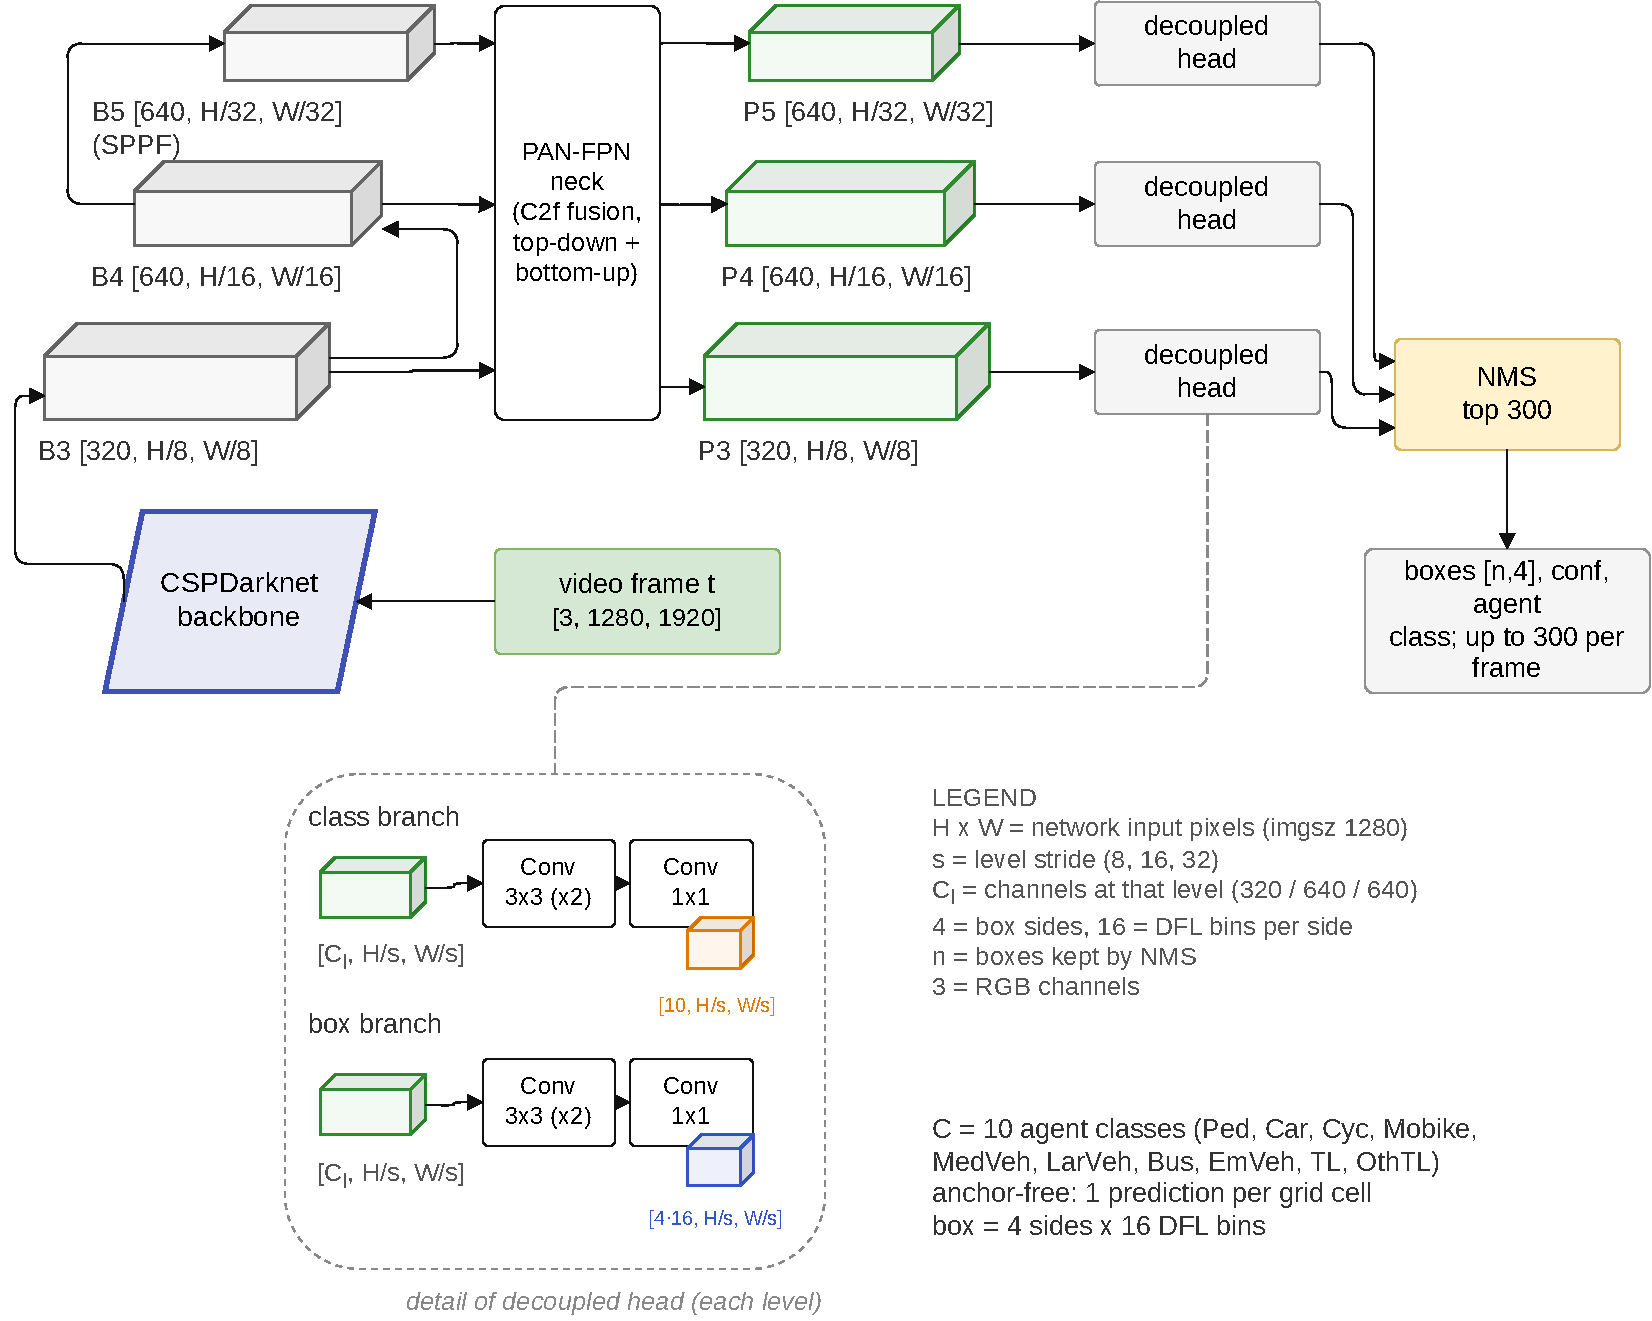
\includegraphics[width=\textwidth,height=0.68\textheight,keepaspectratio]{Fig/yolov8x.pdf}
\caption{YOLOv8x agent-detector architecture.}
\label{fig:4}
\end{figure}

For each YOLO box, Stage 1 finds the baseline detection with highest IoU on the same frame. If IoU is at least 0.5, the action, location, duplex, and triplet scores are copied from that detection. Otherwise, those scores remain zero. Matching is performed independently per YOLO box and does not impose a one-to-one assignment. YOLO supplies the emitted agentness and agent-class detections. No new score-transfer module is trained. Transferred event scores are emitted directly, without multiplication by YOLO confidence.

Across the 36,717 shared frames, approximately 40.6\% of 6,163,968 YOLO candidates find a qualifying baseline match. This is the proportion of candidates that receive transferred event scores; it is not ground-truth recall or classification accuracy. Figure~\ref{fig:score-transfer-limit} illustrates why: an unmatched YOLO box has no baseline event-score source, so its transferred action, location, duplex, and triplet values remain zero. A correctly localized object can consequently lack useful event predictions. The next stage addresses this dependence by extracting a feature at every candidate box.

\begin{figure}[htbp]
\centering
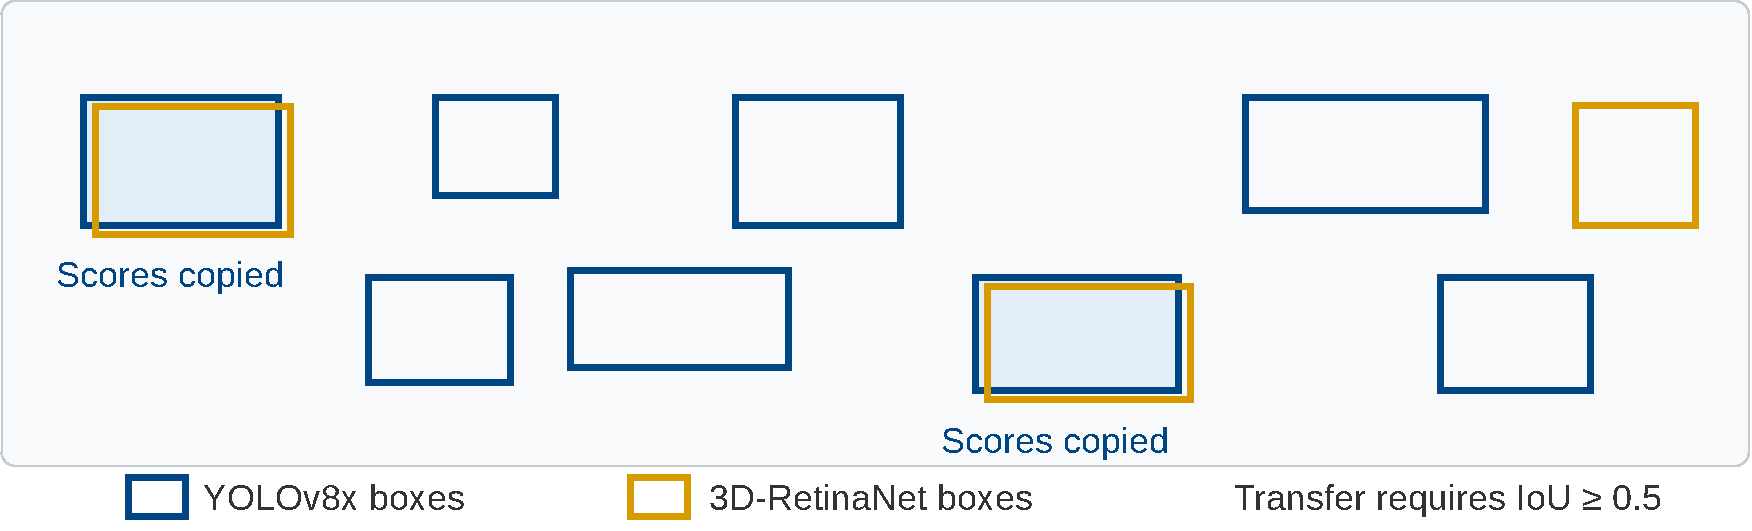
\includegraphics[width=\textwidth,height=0.60\textheight,keepaspectratio]{Fig/score-transfer-limit.pdf}
\caption[The event-score coverage limitation of overlap transfer.]{The event-score coverage limitation of overlap transfer. The boxes illustrate matched and unmatched candidates; their counts do not represent the measured match rate.}
\label{fig:score-transfer-limit}
\end{figure}

Figure~\ref{fig:5} summarizes the score-transfer path: overlap matching determines whether a YOLO candidate receives the baseline’s event scores.

\begin{figure}[htbp]
\centering
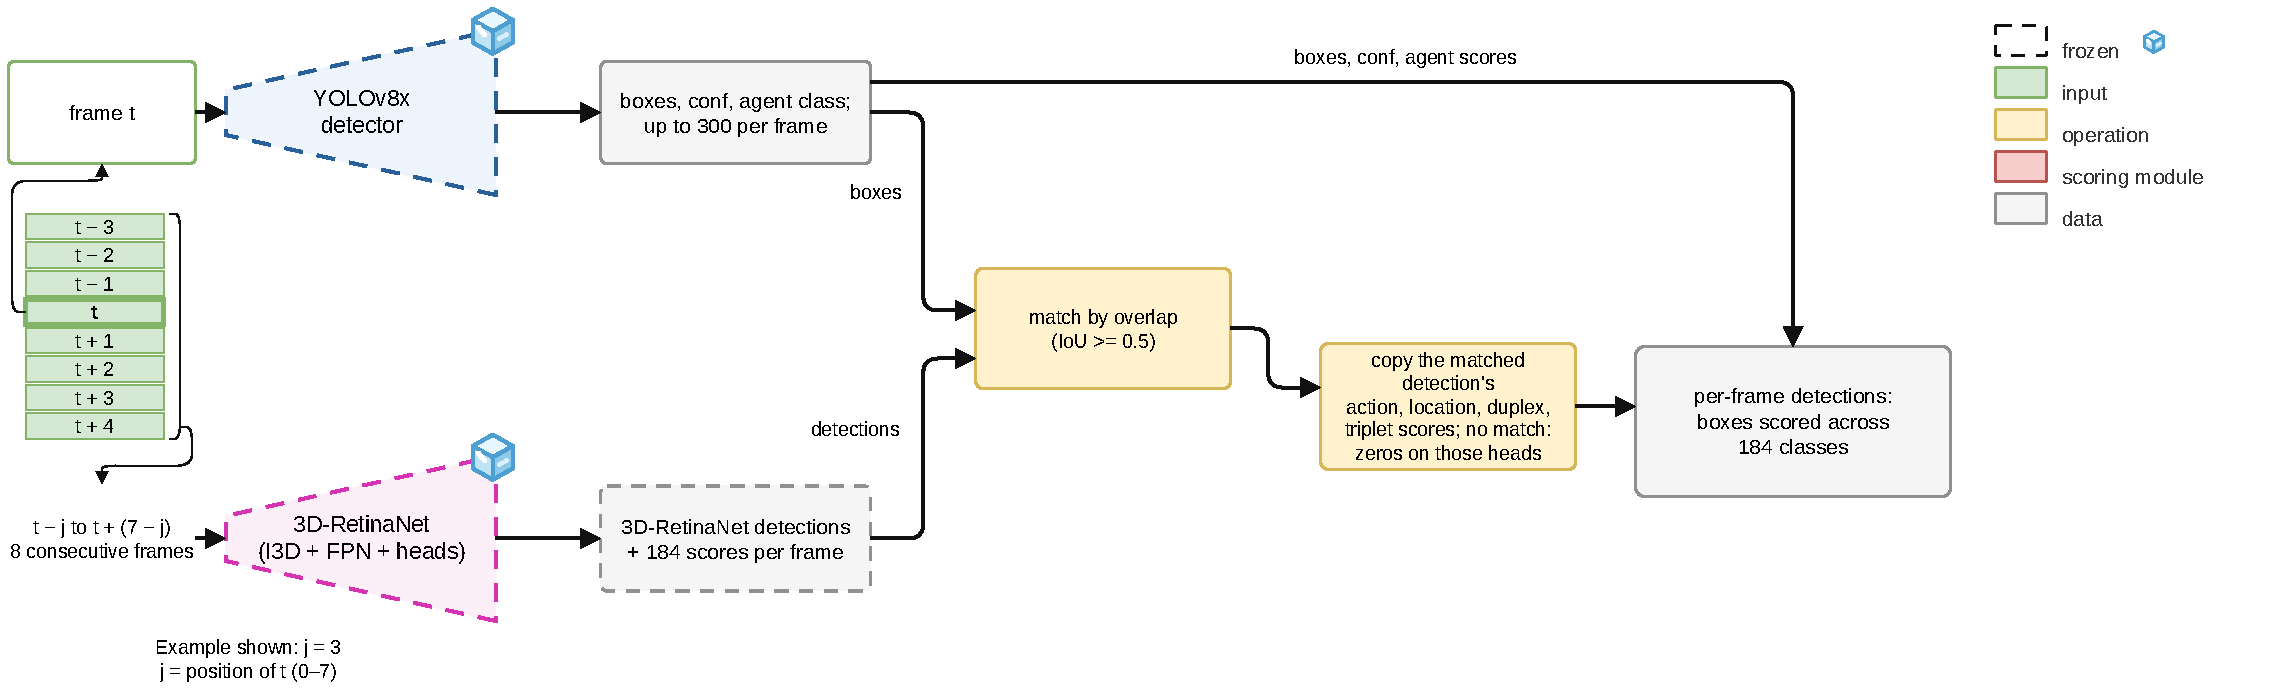
\includegraphics[width=\textwidth,height=0.68\textheight,keepaspectratio]{Fig/stage1-transfer.pdf}
\caption{Stage 1 detector replacement and overlap-based score transfer.}
\label{fig:5}
\end{figure}

\section{Direct Region Features and Event Classification}

Stage 2 replaces overlap-based score transfer with feature extraction at each YOLO box. Figure~\ref{fig:stage2-roialign} shows the detector--classifier path: the detector and video backbone remain frozen while the event head is trained.

\begin{figure}[htbp]
\centering
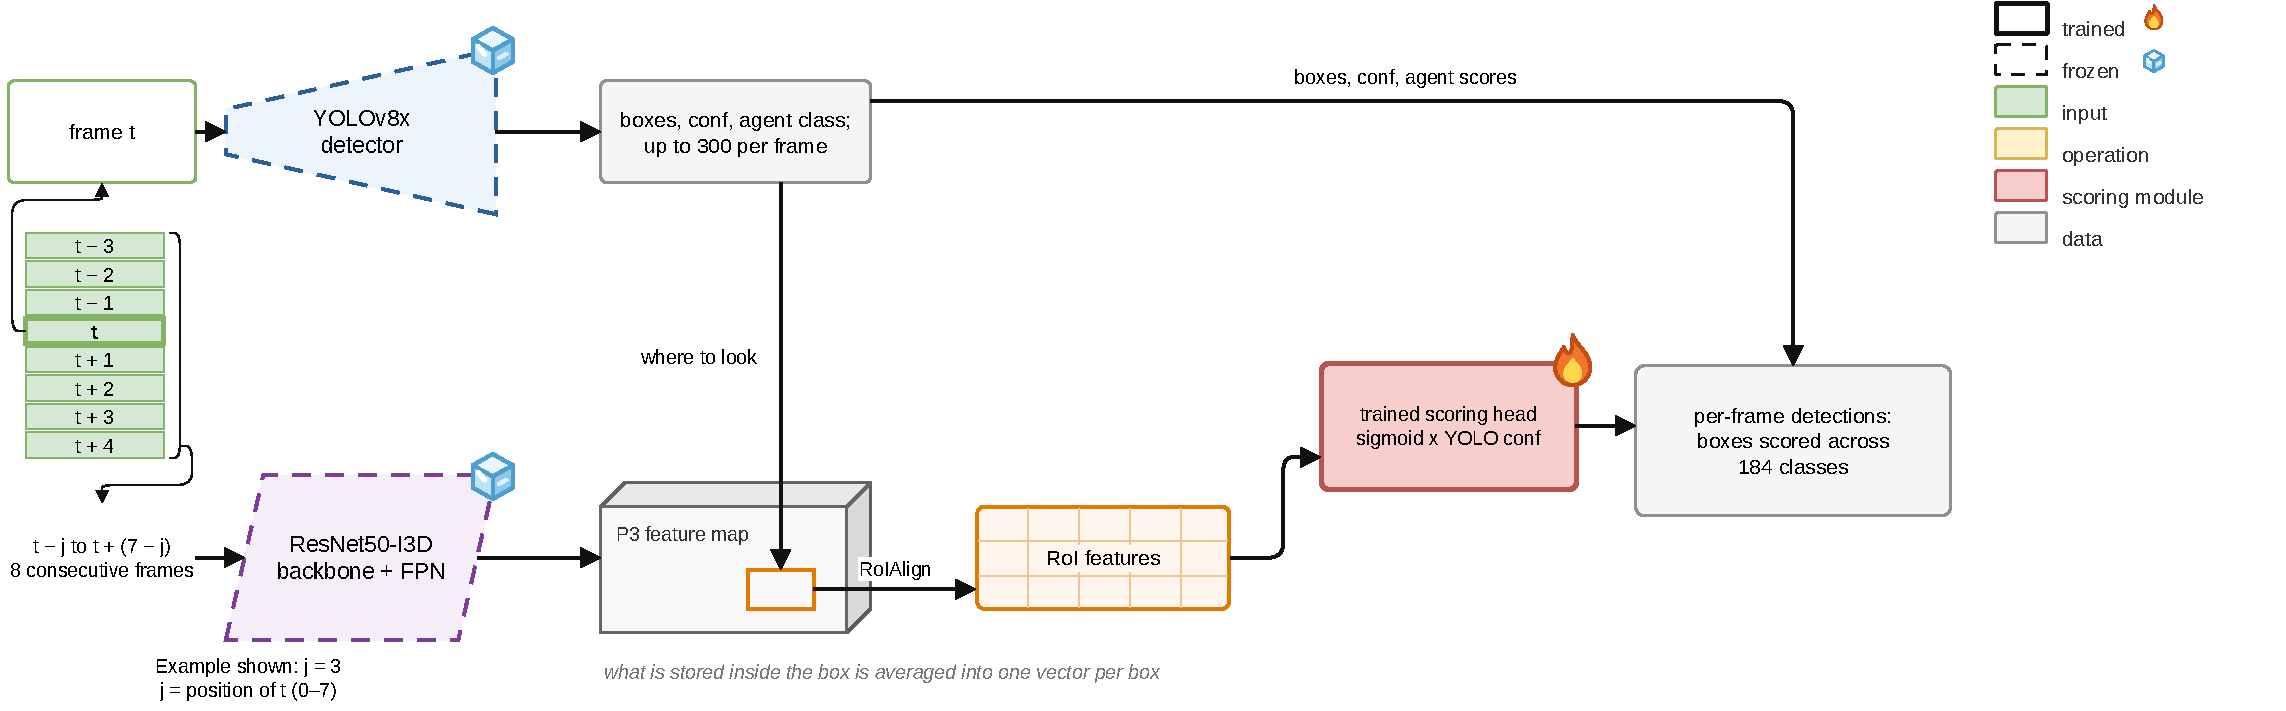
\includegraphics[width=\textwidth,height=0.60\textheight,keepaspectratio]{Fig/stage2-roialign.pdf}
\caption[Stage 2 direct region-feature classification.]{Stage 2 direct region-feature classification.}
\label{fig:stage2-roialign}
\end{figure}

Stage 2 reads the frozen I3D/FPN P3 feature map at every YOLO box using RoIAlign \cite{mask-rcnn}. Boxes are mapped into feature-map coordinates and pooled to one 256-dimensional vector at the corresponding frame. Temporal interpolation aligns the feature map with the clip length when needed. Unlike score transfer, this procedure can obtain a feature at a location that the baseline detection head did not select.

Figure~\ref{fig:roi-align} expands this operation. The implementation rescales box coordinates to the P3 grid, selects the feature slice for the target frame, and applies aligned RoIAlign with a single spatial output bin. Bilinear sampling and averaging produce one 256-dimensional vector for each box. The illustrated sample locations explain the pooling operation; they are not additional detections. Because the map was produced from a video clip, the regional feature can incorporate temporal context even though the readout is associated with one target frame \cite{mask-rcnn}.

\begin{figure}[htbp]
\centering
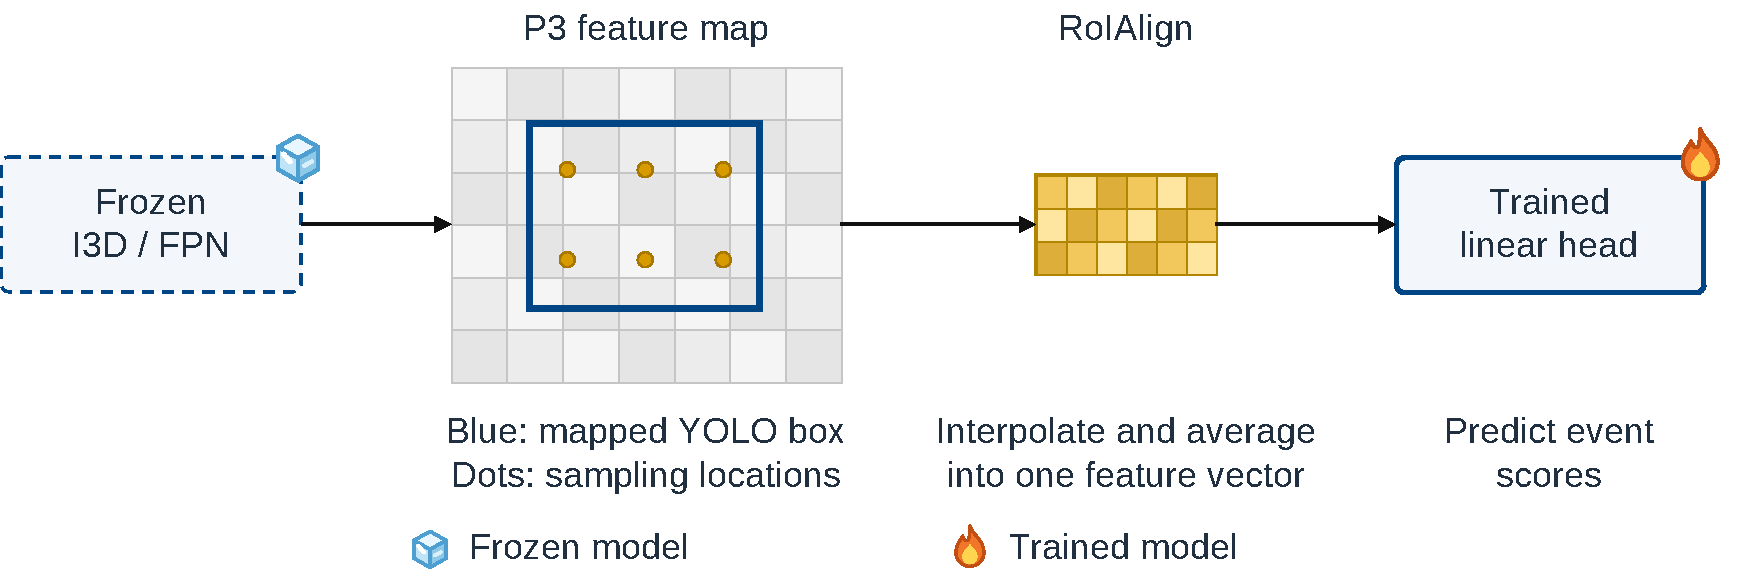
\includegraphics[width=\textwidth,height=0.60\textheight,keepaspectratio]{Fig/roi-align.pdf}
\caption[RoIAlign extraction at a proposed box.]{RoIAlign extraction at a proposed box.}
\label{fig:roi-align}
\end{figure}

A linear layer maps each vector to 184 logits. Training uses ground-truth boxes with multi-hot targets, random background boxes, and an additional set of YOLO background candidates. Background targets are zero across the output vector. The reported configuration uses focal classification loss with class-dependent alpha weights and focusing parameter \(\gamma = 2\) \cite{focal-loss}. The optional logical-penalty coefficient is zero in this configuration.

During evaluation, the head’s action, location, and composition sigmoids are multiplied by YOLO confidence. For a candidate with confidence q and raw class score p, the emitted score is qp. This gate affects detection ranking; it should not be interpreted as proof of calibrated probability. YOLO remains responsible for the emitted agentness and hard agent class. The Stage 1-to-2 transition changes feature access, the trained classifier, and confidence gating; it is not a feature-access-only ablation.

\section{Stacked Composition Learning}

Stage 3 keeps the Stage 2 feature extractor and full-data head fixed at evaluation. It concatenates 49 ungated primitive scores with the 256-dimensional pooled feature, producing a 305-dimensional input. A two-layer MLP, Linear(305,512) \(\rightarrow\) ReLU \(\rightarrow\) Linear(512,135), predicts 49 duplex and 86 triplet logits. Its sigmoid outputs replace only the composition columns.

The MLP is trained using video-grouped, two-fold out-of-fold predictions. These internal training folds do not replace the held-out validation split; the procedure is detailed below.

At evaluation, the full-training-data head supplies primitive predictions. The MLP receives raw, ungated sigmoids and the pooled feature. Its composition scores are gated by YOLO confidence only at emission. This ordering matches the representation used to train the MLP. Action and location pass through from Stage 2, and YOLO boxes and agent outputs remain unchanged.

Figure~\ref{fig:out-of-fold} details the training-only procedure, following the principle of stacked generalization \cite{stacking}. Training videos are assigned to two folds. A temporary linear head trained on fold A supplies predictions for fold B, and the head trained on fold B supplies predictions for fold A. The composition MLP therefore learns from predictions on videos excluded from the corresponding temporary head\textquotesingle{}s training set. Grouping by video prevents adjacent frames from being split between the two folds. The held-out designation applies to these temporary heads; the visual backbone is a shared frozen representation. The temporary heads are discarded after generating the MLP training inputs.

\begin{figure}[htbp]
\centering
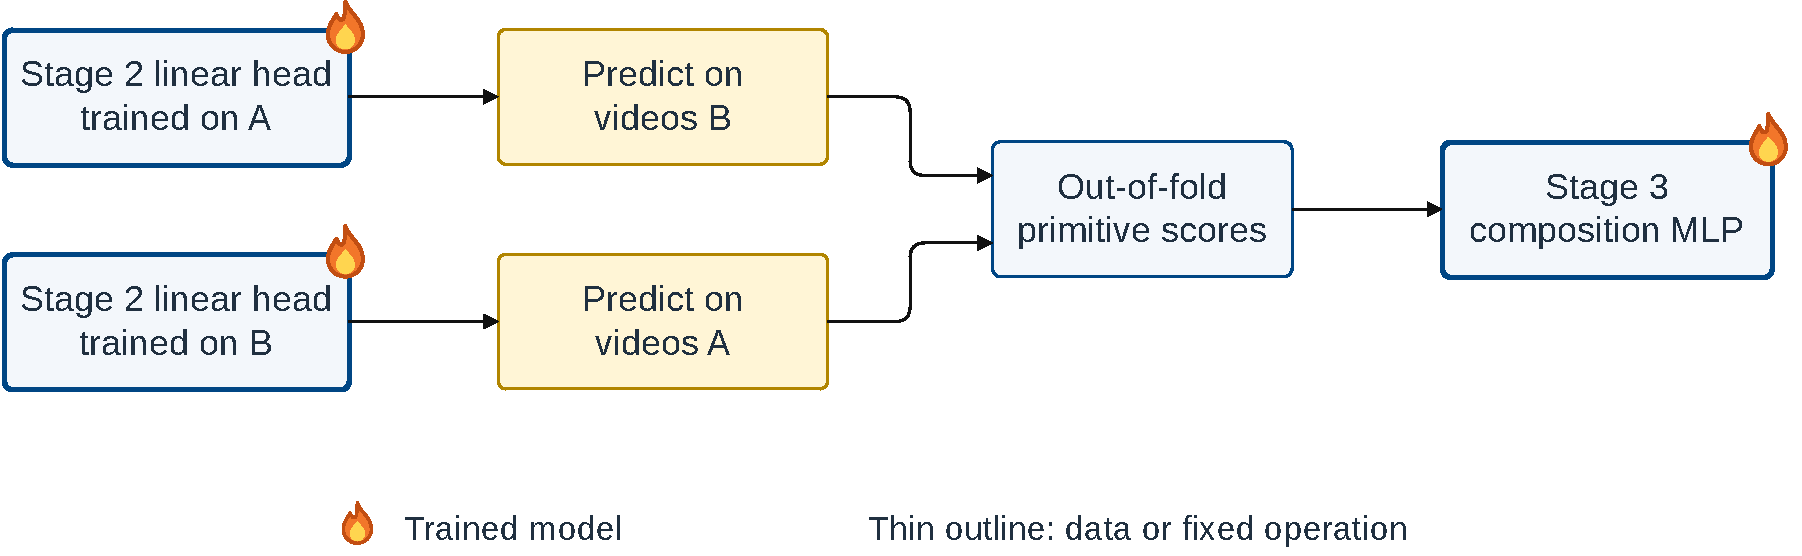
\includegraphics[width=\textwidth,height=0.60\textheight,keepaspectratio]{Fig/out-of-fold.pdf}
\caption[Video-grouped out-of-fold inputs for composition learning.]{Video-grouped out-of-fold inputs for composition learning, adapted from the stacking principle \cite{stacking}. A and B are folds of the training split.}
\label{fig:out-of-fold}
\end{figure}

Figure~\ref{fig:composition-detail} distinguishes learning a composition from replacing the entire prediction vector. The MLP receives 49 ungated scores---agentness plus agent, action, and location---together with 256 regional features. Its 135 outputs replace only the 49 duplex and 86 triplet entries. The feature input supplies visual evidence when primitive scores alone are ambiguous; retaining the remaining outputs makes the Stage 2-to-3 comparison specific to composition learning.

\begin{figure}[htbp]
\centering
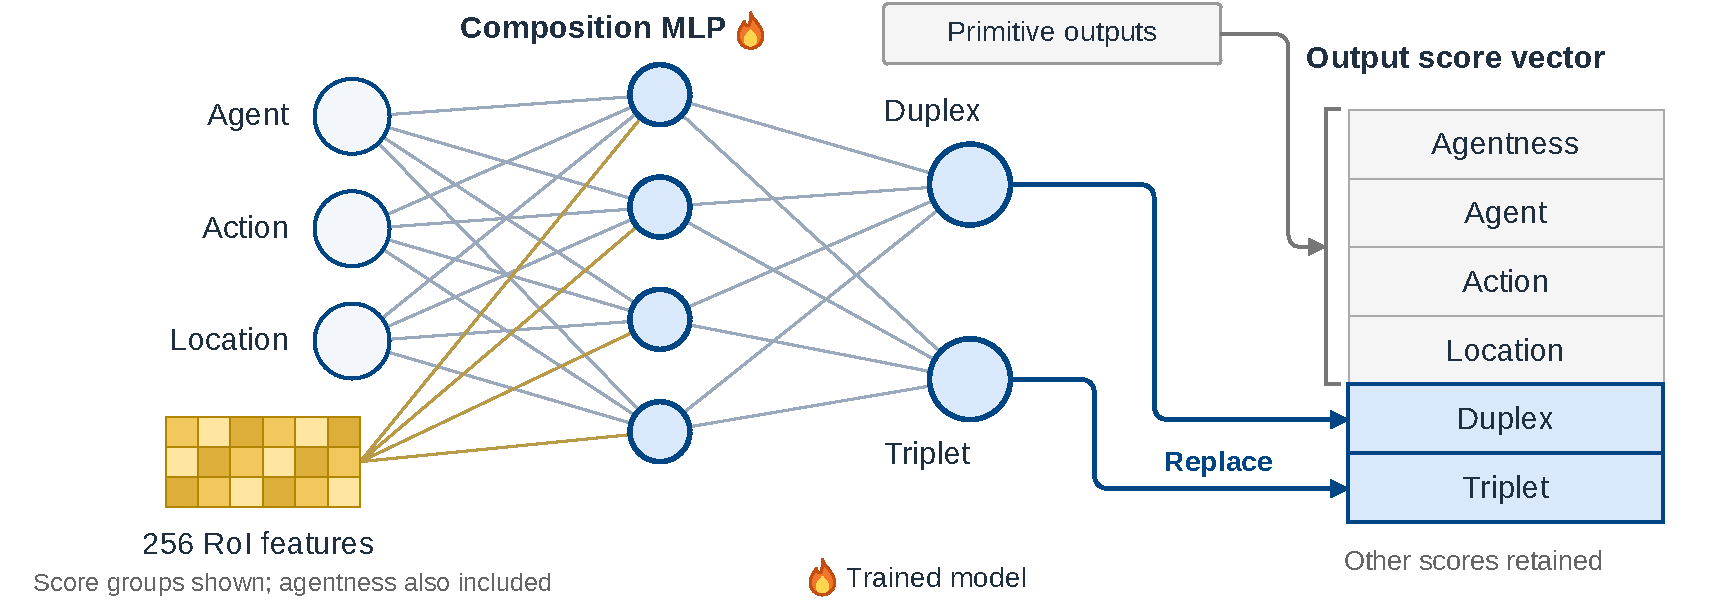
\includegraphics[width=\textwidth,height=0.60\textheight,keepaspectratio]{Fig/composition-detail.pdf}
\caption[Composition learning and selective output replacement.]{Composition learning and selective output replacement.}
\label{fig:composition-detail}
\end{figure}

The output vocabulary includes only the valid benchmark compositions. A nonexistent tuple has no dedicated output column. This vocabulary restriction does not guarantee agreement between independently scored primitives and compositions; cross-head consistency is a separate property.

Figure~\ref{fig:6} summarizes the completed Stage 3 architecture. Its composition module builds on the Stage 2 representation while preserving boxes and primitive outputs, providing the reference point for the results in Chapter 4.

\begin{figure}[htbp]
\centering
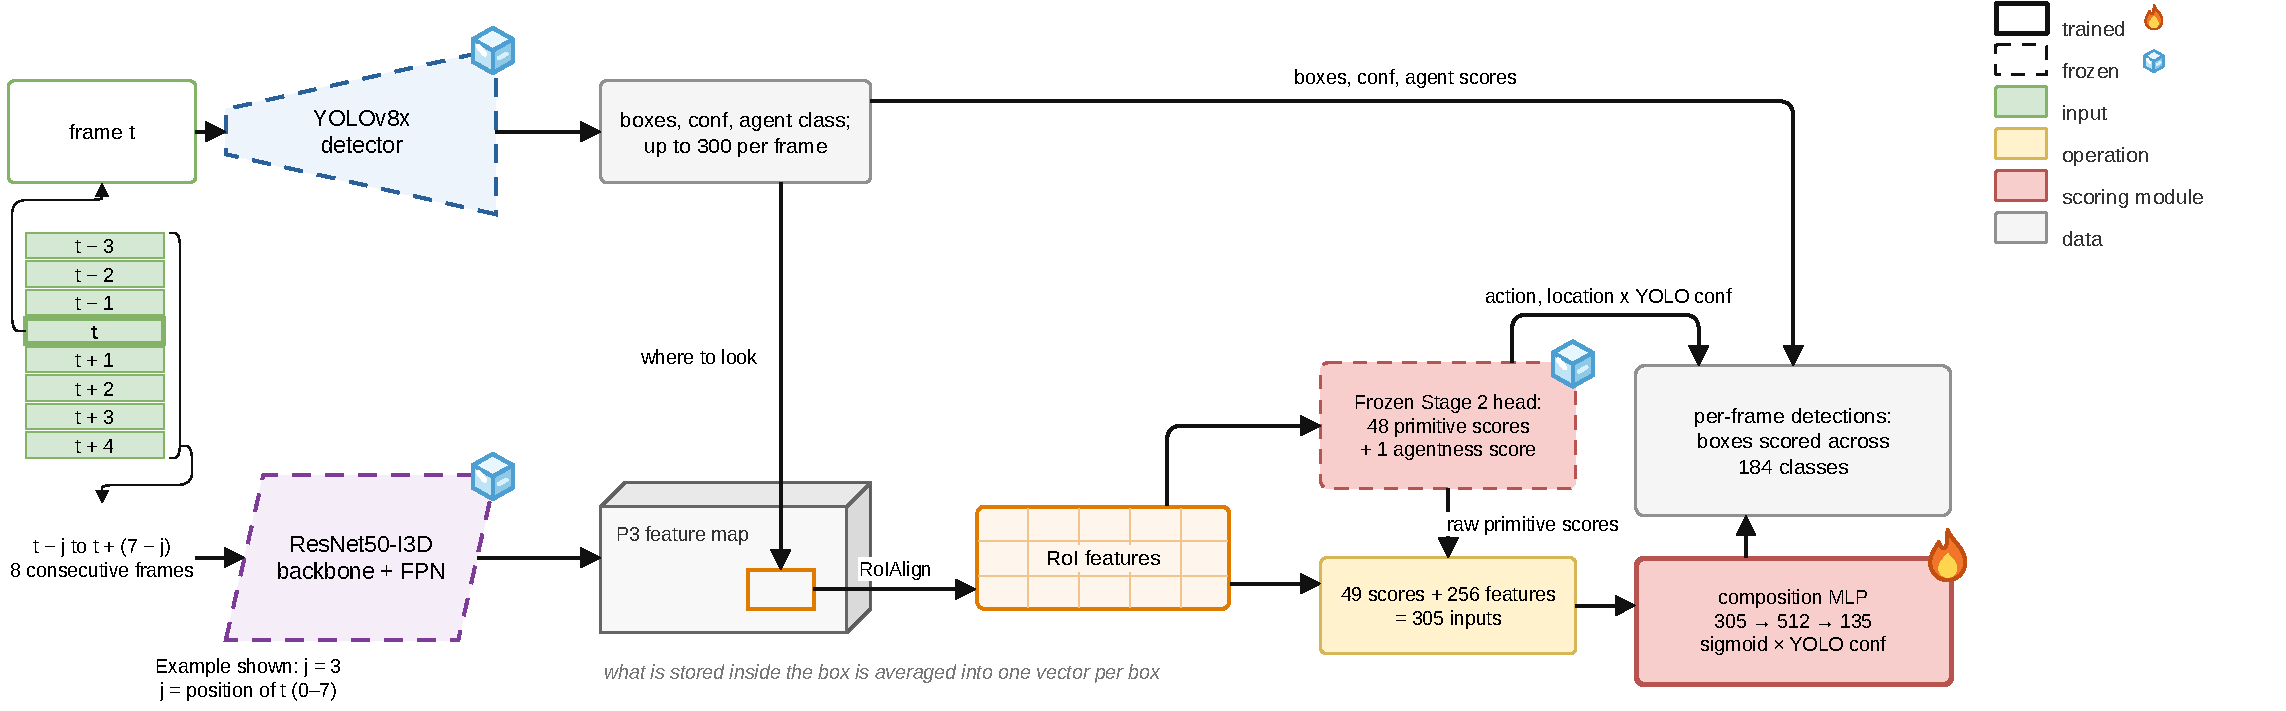
\includegraphics[width=\textwidth,height=0.68\textheight,keepaspectratio]{Fig/stage3-composition.pdf}
\caption{Completed Stage 3 learned-composition architecture.}
\label{fig:6}
\end{figure}

\section{Reproducibility and Label Integrity}

The source implementation fixes the 184-column ordering across frozen feature outputs, prediction heads, and evaluation. YOLO boxes are normalized coordinates; baseline boxes stored in an 840 \(\times\) 600 convention are converted before overlap calculations. These conventions are necessary for meaningful box matching and score assembly.

Valid compositions are derived from benchmark label names and the verified constraints file. The legacy duplex\_childs and triplet\_childs arrays are not used as authoritative mappings. Experiment records will retain the exact class order, candidate and feature identities, seeds, and evaluation manifests.
